\chapter{Galaxy Contamination}
\label{ch8}

When looking at our ALMA images in POLI, we noticed a faint object, that we think could be a background galaxy. I wanted to apply methods similar to those in \cite{sadavoy_dust_2019}. This consists of 



\begin{figure*}[h]
  \centering
  % First figure
  \begin{minipage}{0.48\textwidth}
    \centering
    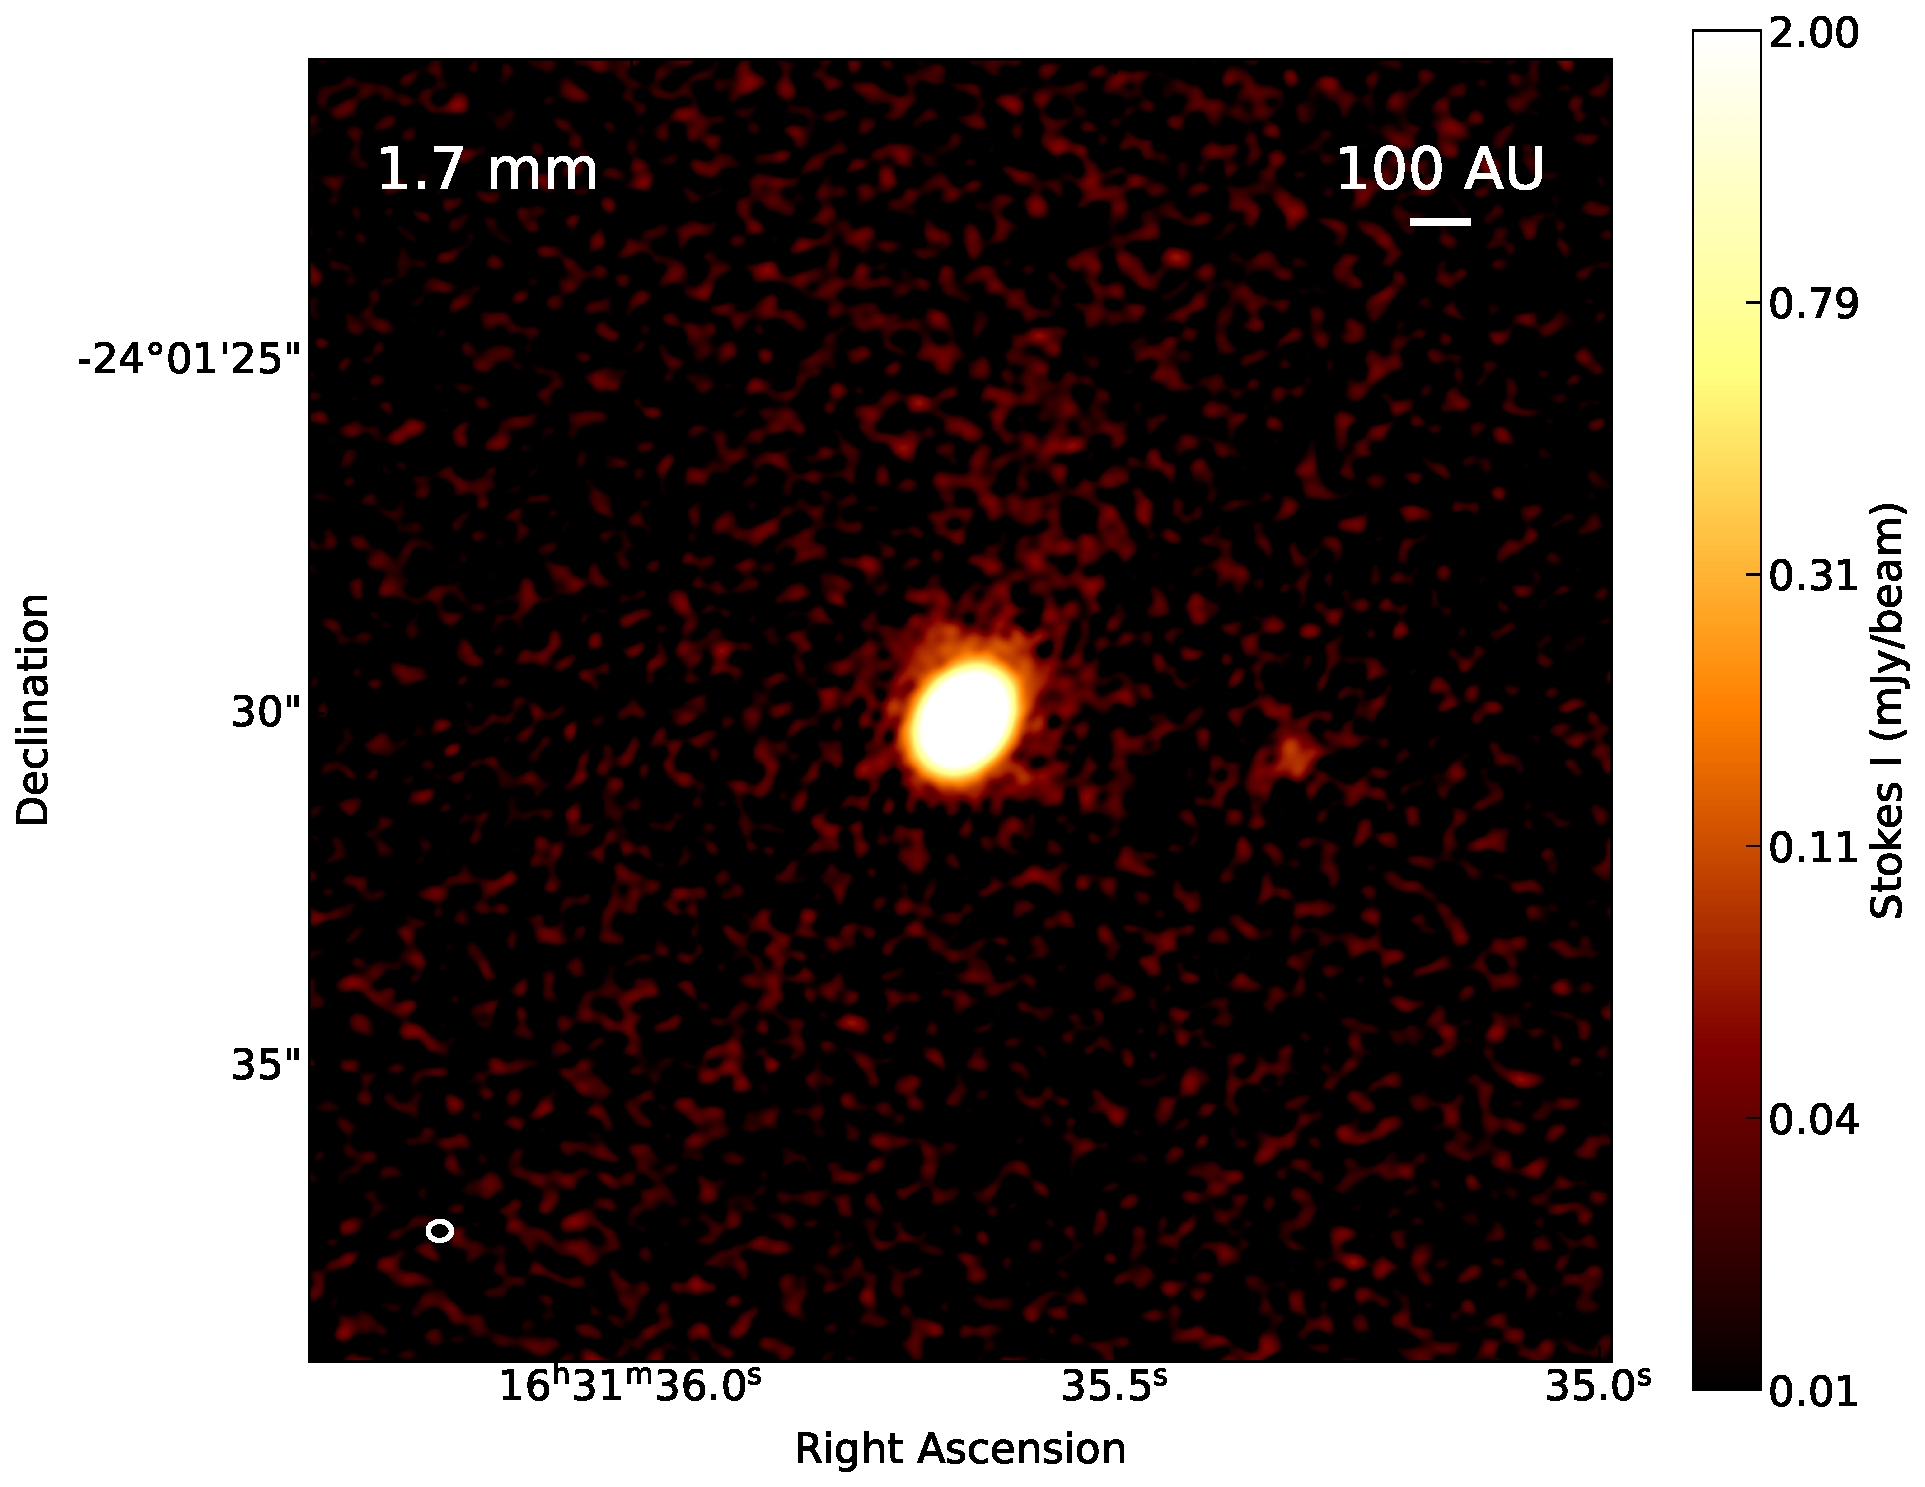
\includegraphics[width=\linewidth]{WRITEUP_AND_IMAGES/IMAGES/WRITEUP/GalaxyContamination/StokesI_BAND5.pdf}
    \caption{Galaxy Contamination of Band 5. Note that Stokes I is cutoff for visualization.}
    \label{fig: GC_POLI_Band5}
  \end{minipage}%
  \hfill
  % Second figure
  \begin{minipage}{0.48\textwidth}
    \centering
    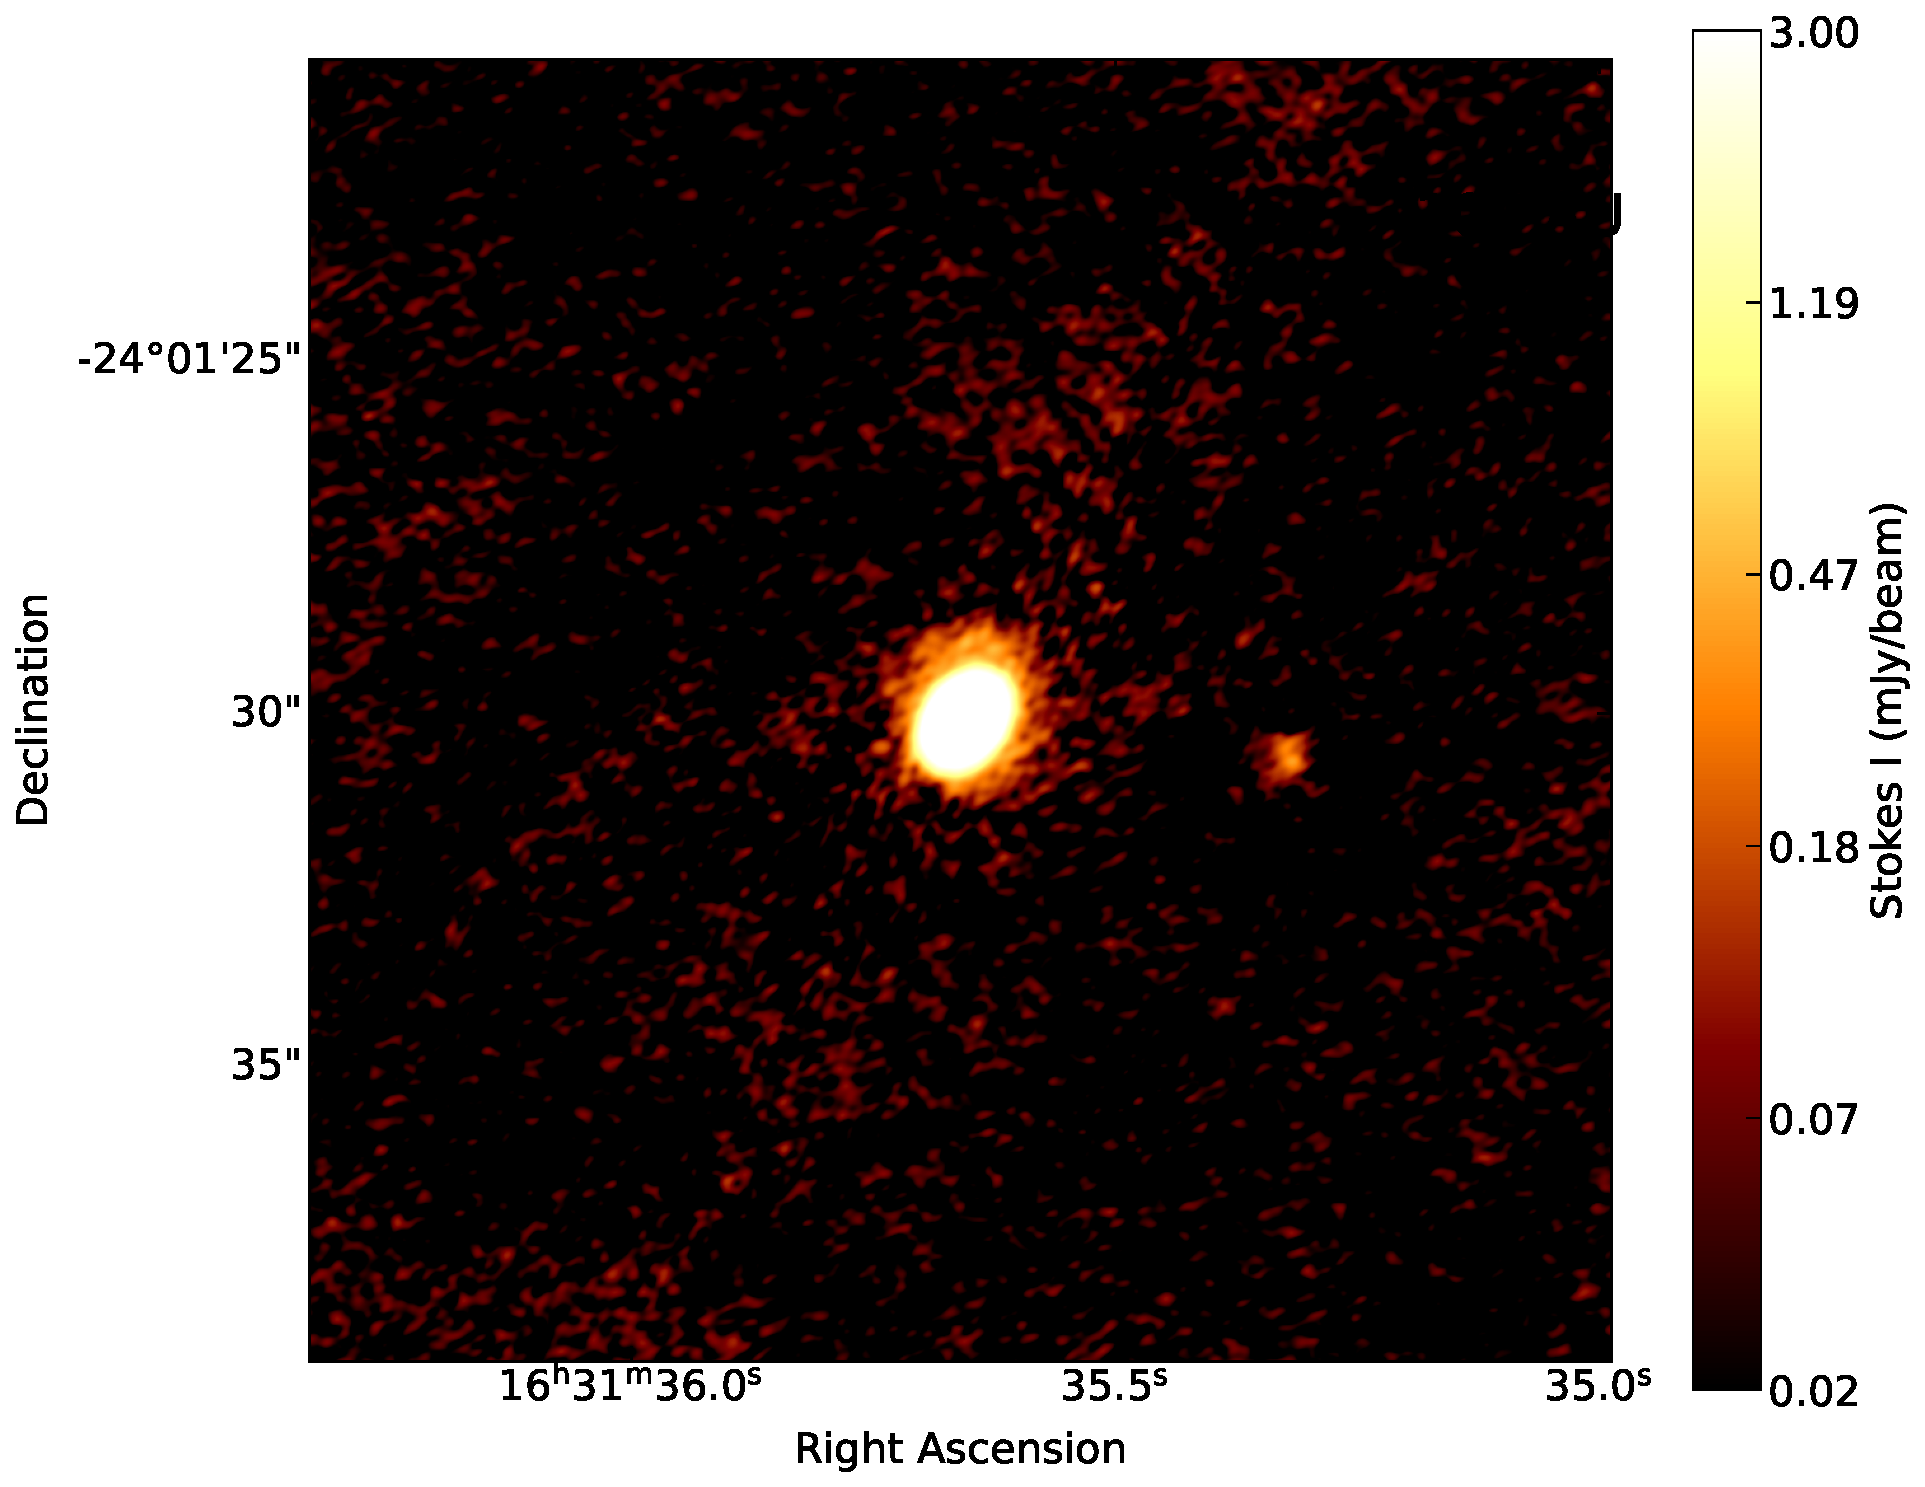
\includegraphics[width=\linewidth]{WRITEUP_AND_IMAGES/IMAGES/WRITEUP/GalaxyContamination/StokesI_BAND7.pdf}
    \caption{Same as Figure \ref{fig: GC_POLI_Band5}, but for Band 7. Note that Stokes I is cutoff for visualization.}
    \label{fig: GC_POLI_Band7}
  \end{minipage}
\end{figure*}






IN the paper \cite{Sadavoy_2019}, the topic of galaxy contamination was covered. 

I used the primary beam file provided to replicate Figures 11 and 12 from the paper. I then wanted to use these methods to apply them to my source. 


My source is visible at Band 5 and Band 7. However, due to <some things> Band 5 is not well studied in number count statistics, so I cannot repliate these methods for Band 7. However, it works for Band 7.

In \cite{Sadavoy_2019} they used a Schechter function:
\begin{equation}
    \frac{dN}{dS} = \text{deg}^{-2}\left(\frac{S}{S_0}\right)^{-\alpha} \exp\left(\frac{S}{S_0}\right).
\end{equation}


I did not do the fit myself but Band 7 was fit using a double-power law function with a form slightly different from the Schechter function with the form of:
\begin{equation}
    \frac{dN}{dS} = \text{deg}^{-2}\left(\frac{S}{S_0}\right)^{-\alpha} \exp\left(\frac{S}{S_0}\right).
    \label{eq: double_power_law}
\end{equation}

\noindent where $N_0$, $S_0$ and $\alpha$ and $\beta$ are the two power law slopes. The corresponding values are found in Table \ref{tab: GC_parameter_table}.



\begin{table}[h!]
\centering
\caption{Best-fit parameters of Equation~\ref{eq:double_power_law} (differential number counts) from \cite{Stach_2018} for Band~7 ($\lambda = 0.870$ mm).}
\label{tab: GC_parameter_table}
\begin{tabular}{cccc}
\toprule
\textbf{$N_0$} & \textbf{$S_0$} & \textbf{$\alpha$} & \textbf{$\beta$} \\
\midrule 
N & S & a & b \\
\bottomrule
\end{tabular}
\end{table}


The S/N of the source in Band 7 is approx. 9.4. The distance to the source is 4.75 arcsec. At the S/N ratio of 5, 9, 20 respectively are 12.03\%, 7.15\% and 3.12\%.




\begin{figure*}[h]
  \centering
  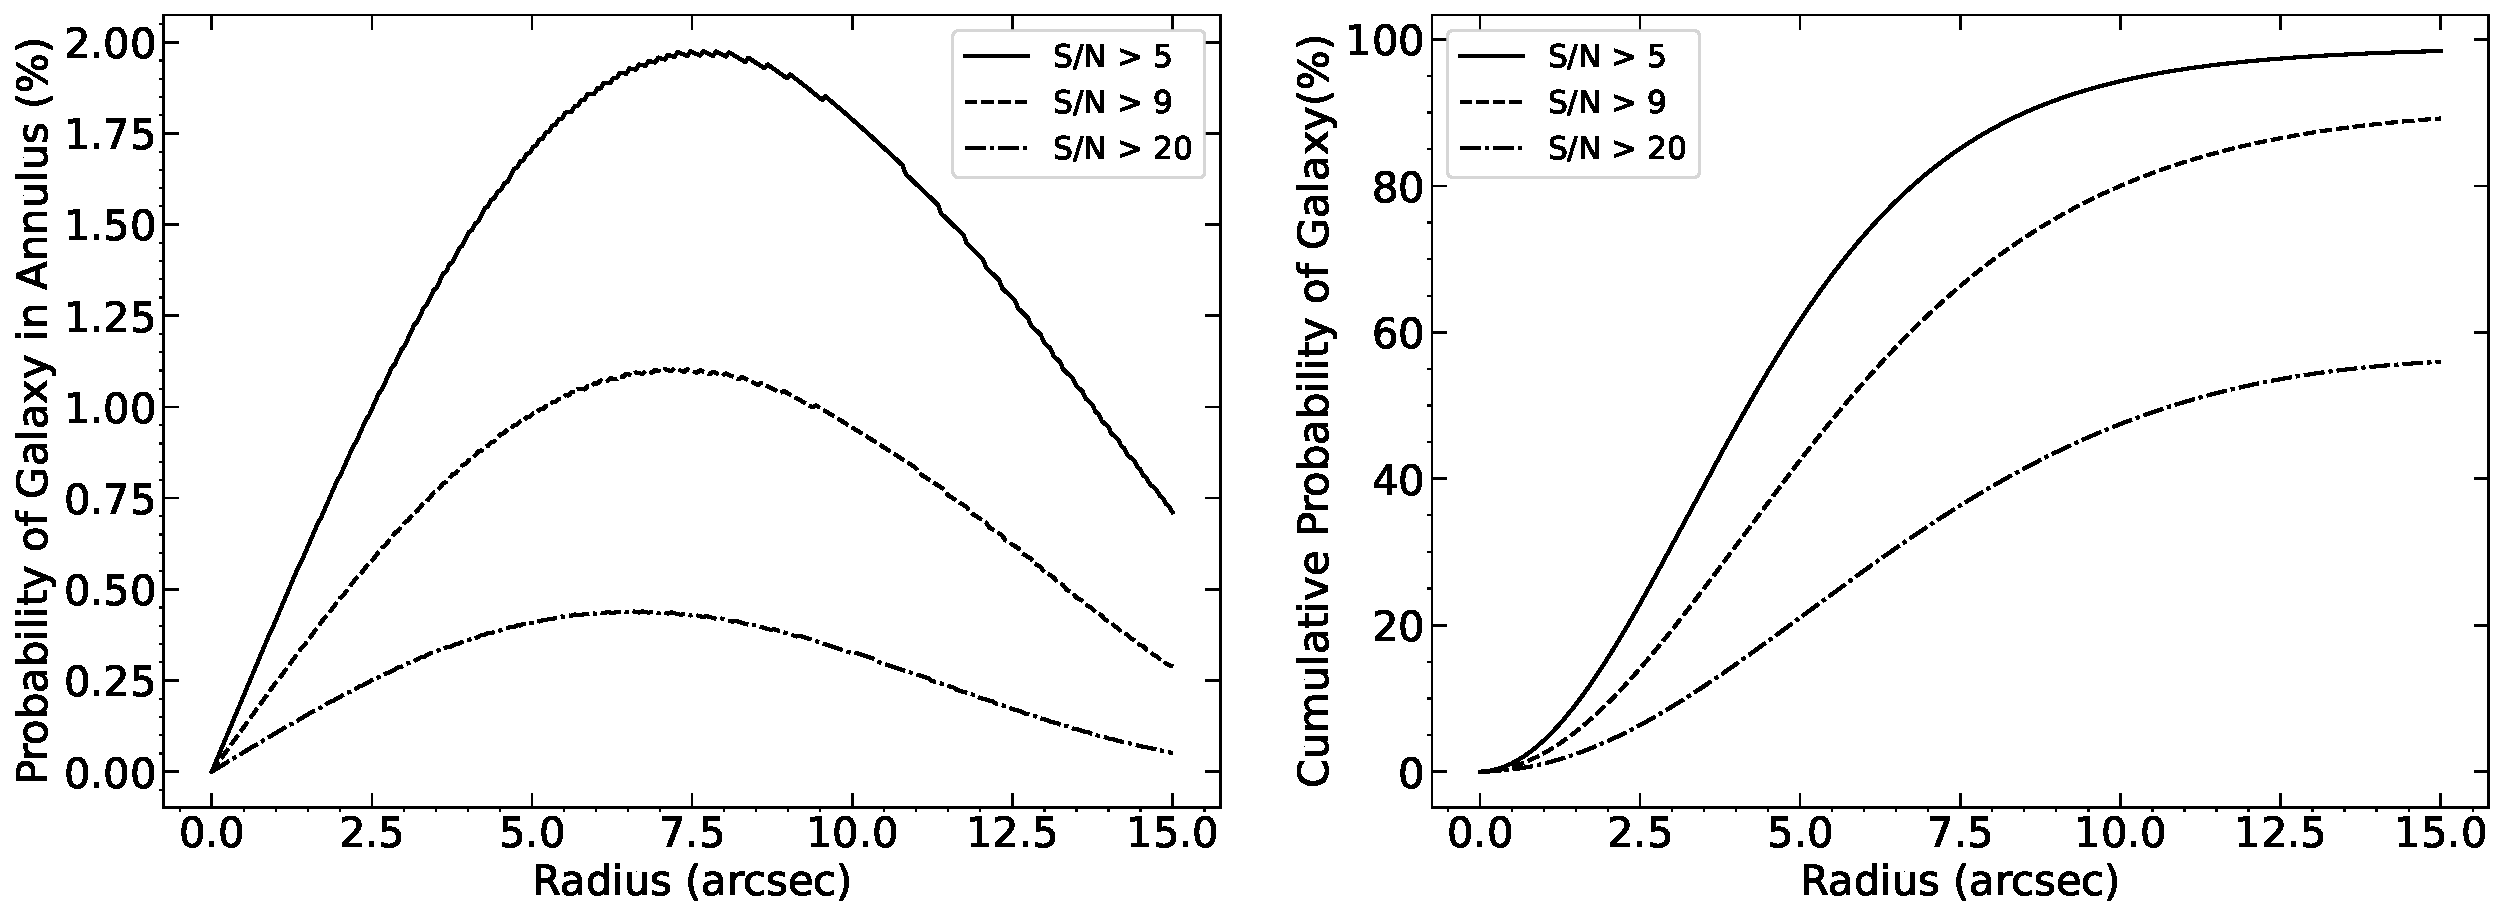
\includegraphics[width=0.8\textwidth]{WRITEUP_AND_IMAGES/IMAGES/WRITEUP/GalaxyContamination/Probabilities_Band7.pdf}
  \caption{Galaxy contamination for Band 7.}
  \label{fig: GalaxyContamination_Prob_B7}
\end{figure*}



